%------------------------------------------------------------------------------
% Copyright (c) 1991-2014, Xavier Leroy and Didier Remy.
%
% All rights reserved. Distributed under a creative commons
% attribution-non-commercial-share alike 2.0 France license.
% http://creativecommons.org/licenses/by-nc-sa/2.0/fr/
%
% Translation by Daniel C. Buenzli
% 英語版の日本語への翻訳: Yuki (github: inzkyk)
%------------------------------------------------------------------------------

% \chapter{\label{sec/pipes}Classical inter-process communication: pipes}
\chapter{\label{sec/pipes}古典的なプロセス間通信: パイプ}

\cutname{pipes.html}

% So far, we have learned how to manage processes and how they can communicate
% with the environment by using files. In the remainder of the
% course we see how processes running in parallel can cooperate by
% communicating among themselves.
これまでは見てきたのはプロセスを管理する方法とファイルを使って外部環境と通信する方法です。コースの残りの部分では、並列に実行されるプロセス同士がコミュニケーションを取りながら協調する方法を見ていきます。

% \section{Pipes}
\section{パイプ}

% Regular files are not a satisfactory communication medium for processes
% running in parallel. Take for example a reader/writer situation in
% which one process writes data and the other reads them. If a file is used
% as the communication medium, the reader can detect that the file
% does not grow any more (\ml+read+ returns zero), but it does not know
% whether the writer is finished or simply busy computing
% more data. Moreover, the file keeps track of all the data transmitted,
% requiring needless disk space.
並列に実行されるプロセス同士がやり取りを行う手段として通常ファイルは十分ではありません。例えば一つのファイルにあるプロセスが書き込み、その内容を別のプロセスが読み込む状況を考えてみてください。やり取りの手段としてファイルを使った場合、読み込み側はファイルが終端に達したことを (\ml+read+ が 0 を返すことで)検出することができますが、その理由が書き込みが終わったためなのかそれとも計算に時間がかかっているためなのかを知ることはできません。さらにファイルはやり取りされるデータを全て保持する必要があるので、ディスクを不必要に圧迫します。

% Pipes provide a mechanism suitable for this kind of communication. A
% pipe is made of two file descriptors. The first one
% represents the pipe's output. The second one represents
% the pipe's input. Pipes are created by the system call
% \syscall{pipe}:
パイプはこのようなやり取りに向いた仕組みです。パイプは二つのファイルディスクリプタからなります。一つがパイプの出力を表し、もう一方がパイプの入力を表します。パイプはシステムコール \syscall{pipe} で作成できます。
%
\begin{listingcodefile}{tmpunix.mli}
val $\libvalue{Unix}{pipe}$ : unit -> file_descr * file_descr
\end{listingcodefile}
%
% The call returns a pair \ml+(fd_in, fd_out)+ where \ml+fd_in+ is a
% file descriptor open in \emph{read mode} on the pipe's output and
% \ml+fd_out+ is file descriptor open in \emph{write mode} on the pipe's
% input. The pipe itself is an internal object of the kernel that can
% only be accessed via these two descriptors. In particular, it has no
% name in the file system.
\ml+pipe+ を呼ぶと \ml+(fd_in, fd_out)+ が返ります。\ml+fd_in+ は \emph{読み込み専用} で開かれたパイプの出力を表すファイルディスクリプタで、\ml+fd_out+ は \emph{書き込み専用} で開かれたパイプの入力を表すファイルディスクリプタです。パイプ自身はこれら 2 つのディスクリプタからのみアクセス可能なカーネルの内部オブジェクトです。またパイプはファイルシステムにおいて名前を持ちません。

%% To draw fd and pipes
\tikzset{
  fd/.style={draw,rectangle,inner sep=3mm, rounded corners,
             text width=1.2cm, text centered},
  pipe/.style={draw,cylinder,minimum size=6mm,minimum height=18mm,
               anchor=shape center}}


\begin{myimage}[width="60\%"]
\begin{tikzpicture}
\node (pipe) [pipe] {};
\node (out) [fd, left=of pipe] {\texttt{fd\_out}};
\node (in) [fd, right=of pipe] {\texttt{fd\_in}};
\draw [->] (out) to (pipe);
\draw [->] (pipe) to (in);
\end{tikzpicture}
\end{myimage}

% A pipe behaves like a queue (\emph{first-in, first-out}). The first
% thing written to the pipe is the first thing read from the pipe.
% Writes (calls to \indexvalue{write} on the pipe's input
% descriptor) fill the pipe and block when the pipe is full. They block
% until another process reads enough data at the other end of the pipe
% and return when all the data given to \ml+write+ have been
% transmitted. Reads (calls to \indexvalue{read} on the pipe's output
% descriptor) drain the pipe. If the pipe is empty, a call to \ml+read+
% blocks until at least a byte is written at the other end. It then
% returns immediately without waiting for the number of bytes requested
% by \ml+read+ to be available.
パイプは先入れ先出しのキューのように振る舞います。最初にパイプに書き込んだものが最初にパイプから読み込まれます。書き込み (パイプの入力ディスクリプタへの \ml+write+) はパイプを満たし、パイプが満杯の場合はブロックします。ブロックは他のプロセスがパイプの他方の端から十分な量のデータを読み込むまで続き、\ml+write+ に渡された全てのデータが書き込まれるまで続きます。読み込み (パイプの出力ディスクリプタへの \ml+read+) はパイプの中身を消費します。パイプが空のとき \ml+read+ はパイプの他方の端に少なくとも 1 バイトが書き込まれるまでブロックします。\ml+read+ は要求されたバイト数だけ読み込むまで待つこと無く返ります。

% Pipes are useless if they are written and read by the same process
% (such a process will likely block forever on a substantial write or on
% a read on the empty pipe). Hence they are usually read and written by
% different processes. Since a pipe has no name, one of these processes
% must be created by forking the process that created the pipe. Indeed,
% the two file descriptors of the pipe, like any other file descriptors,
% are duplicated by the call to \indexvalue{fork} and thus refer to the
% same pipe in the parent and the child process.
入出力が同じプロセスから起きるのならばパイプは役に立ちません。そのようなプロセスは大量の書き込みや空のパイプへの読み込みによって永遠にブロックしてしまうからです。そのため普通パイプへの入出力は別々のプロセスが行います。パイプは名前を持たないことから、パイプを利用するプロセスの片方はパイプを作成したプロセスからのフォークによって作られる必要があります。
\begin{example} %The following snippet of code is typical.
次の短いコードは典型的なパイプの使用例です。
%
\begin{lstlisting}
let (fd_in, fd_out) = pipe () in
match fork () with
| 0 -> close fd_in; ... write fd_out buffer1 offset1 count1 ...
| pid -> close fd_out; ... read fd_in buffer2 offset2 count2 ...
\end{lstlisting}
%
% After the \ml+fork+ there are two descriptors open on the pipe's
% input, one in the parent and the other in the child. The same
% holds for the pipe's output.
\ml+fork+ のあとパイプの入力を指すディスクリプタは二つあり、親プロセスと子プロセスが一つづつ持っています。出力用ディスクリプタについても同様です。
%
\begin{myimage}[width="45\%"]
\begin{tikzpicture}
\node (pipe) at (0,0) [pipe] {};
\node (outfather) at (-2,1.5) [fd, font=\fontsize{7pt}{7pt}\selectfont] {\texttt{fd\_out}\\ 親プロセス};
\node (outchild) at (-2,-1.5) [fd, font=\fontsize{7pt}{7pt}\selectfont] {\texttt{fd\_out}\\ 子プロセス};
\node (infather) at (2,1.5) [fd, font=\fontsize{7pt}{7pt}\selectfont] {\texttt{fd\_in}\\ 親プロセス};
\node (inchild) at (2,-1.5) [fd, font=\fontsize{7pt}{7pt}\selectfont] {\texttt{fd\_in}\\ 子プロセス};
\draw [->] (outfather.south) to [bend right=30] (pipe.west);
\draw [->] (outchild.north) to [bend left=30] (pipe.west);
\draw [->] (pipe.east) to [bend right=30] (infather.south);
\draw [->] (pipe.east) to [bend left=30] (inchild.north);
\end{tikzpicture}
\end{myimage}
%
% In this example the child becomes the writer and the parent the
% reader. Consequently the child closes its descriptor \ml+fd_in+ on the
% pipe's output (to save descriptors and to avoid programming
% errors). This leaves the descriptor \ml+fd_in+ of the parent unchanged
% as descriptors are allocated in process memory and after the fork the
% parent's and child's memory are disjoint. The pipe, allocated in system
% memory, still lives as there's still the descriptor \ml+fd_in+ of the
% parent open in read mode on the pipe's output. Following the same
% reasoning the parent closes its descriptor on the pipe's input. The
% result is as follows:
この例では子が書き込みを、親が読み取りを行います。子はパイプの出力 \ml+fd_in+ をクローズしますが、これはディスクリプタを節約しプログラミング上のミスを防ぐためです。ディスクリプタはプロセスのメモリに確保され、フォークすると親子でメモリが別々になるので、子プロセスでディスクリプタをクローズしたとしても親プロセス \ml+fd_in+ はその影響を受けません。パイプはシステムメモリに確保され、親プロセスの \ml+fd_in+ がパイプの出力に読み込みモードで開いている限り生き続けます。同じ理由で親プロセスはパイプの入力へのディスクリプタをクローズします。結果的に以下のような状態となります:

%
\begin{myimage}[width="45\%"]
\begin{tikzpicture}
\node (pipe) at (0,0) [pipe] {};
\node (outchild) at (-2,-1.5) [fd,, font=\fontsize{7pt}{7pt}\selectfont] {\texttt{fd\_out}\\ 子プロセス};
\node (infather) at (2,1.5) [fd, font=\fontsize{7pt}{7pt}\selectfont] {\texttt{fd\_in}\\ 親プロセス};
\draw [->] (outchild.north) to [bend left=30] (pipe.west);
\draw [->] (pipe.east) to [bend right=30] (infather.south);
\end{tikzpicture}
\end{myimage}
%
% Data written by the child on \ml+fd_out+ is transmitted to \ml+fd_in+ in the parent.
子プロセスが \ml+fd_out+ に書き込んだデータは親の \ml+fd_in+ に書き込まれます。
\end{example}
% When all the descriptors on a pipe's input are closed and the pipe is
% empty, a call to \ml+read+ on its output returns zero:
% end of file. And when all the descriptors on a pipe's output are
% closed, a call to \ml+write+ on its input kills the writing
% process. More precisely the kernel sends the signal \ml+sigpipe+ to
% the process calling \ml+write+ and the default handler of this signal
% terminates the process. If the signal handler of \ml+sigpipe+ is
% changed, the call to \ml+write+ fails with an \ml+EPIPE+ error.
パイプの入力へのディスクリプタが全てクローズされかつパイプが空のとき、パイプの出力への \ml+read+ は 0 (ファイルの終端) を返します。パイプの出力へのディスクリプタが全てクローズされているとき、パイプの入力への \ml+write+ は書き込みプロセスを終了させます。より正確に言うと、カーネルが \ml+write+ を呼んだプロセスに \ml+sigpipe+ シグナルを送り、このシグナルのデフォルトの動作がプロセスの終了です。\ml+sigpipe+ シグナルのハンドラが変更していた場合は、 \ml+write+ は \ml+EPIPE+ エラーを出して失敗します。

% \section{\label{ex/crible}Complete example: parallel sieve of Eratosthenes}
\section{\label{ex/crible}完全な例: 並列エラトステネスのふるい}

% This is a classic example of parallel programming. The task of the
% program is to enumerate the prime numbers and display them
% interactively as they are found. The idea of the algorithm is as
% follows. A process enumerates on its output the integers from 2 onwards. We
% connect this process to a \quotes{filter} process that reads an
% integer $p$ on its input and displays it.
これは並列プログラミングの古典的な例です。ここで扱うのは素数を順に列挙しながら見つかった順にインタラクティブに表示するという問題です。アルゴリズムのアイデアは次のようなものです。あるプロセスが 2 から順に整数を出力します。このプロセスに整数 $p$ を一つ受け取って表示する別の \emph{フィルター} プロセスをつなげます。

\tikzset{process/.style={draw,rectangle,inner sep=2mm, rounded corners,
             text width=1cm, minimum height=1cm, text
             centered,font=\small},
         output/.style={font=\small,above}}

\begin{myimage}[width="38\%"]
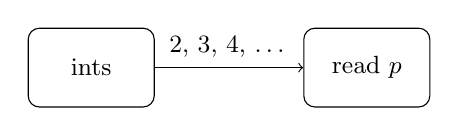
\begin{tikzpicture}
\node (intgen) at (0,0) [process] {ints};
\node (read) at (3.5,0) [process] {read $p$};
\draw [->] (intgen) to node [output] {2, 3, 4, \ldots} (read);
\end{tikzpicture}
\end{myimage}
%
% Therefore, the first filter process reads $p=2$. Then it creates a new
% filter process connected to its output and filters out the multiples
% of $p$ it gets on its input; all numbers it reads that are not a
% multiple of $p$ are rewritten on its output.
最初のフィルタープロセスは 2 を最初に受け取ることから $p=2$ となります。このプロセスは自分の出力と接続した新しいフィルタープロセスを作成します。そして新しいプロセスに $p$ の倍数でない整数を入力します。
%
\begin{myimage}[width="65\%"]
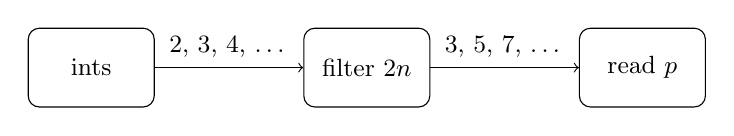
\begin{tikzpicture}
\node (intgen) at (0,0) [process] {ints};
\node (filter2) at (3.5,0) [process] {filter $2n$};
\node (read) at (7,0) [process] {read $p$};
\draw [->] (intgen) to node [output] {2, 3, 4, \ldots} (filter2);
\draw [->] (filter2) to node [output] {3, 5, 7, \ldots} (read);
\end{tikzpicture}
\end{myimage}
%
% Hence the next process reads $p=3$, which it displays and then starts
% to filter multiples of 3, and so on.
新しいフィルタープロセスは 3 を最初に受け取るので $p=3$ となります。このプロセスは 3 の倍数をフィルターし、同じことが次のプロセスへと続きます。
%
\begin{myimage}[width="100\%"]
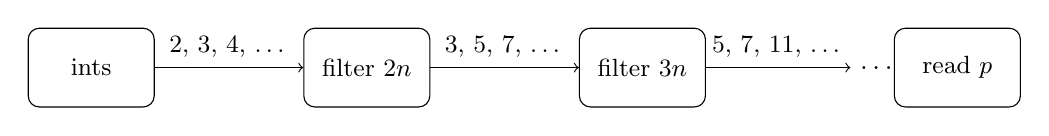
\begin{tikzpicture}
\node (intgen) at (0,0) [process] {ints};
\node (filter2) at (3.5,0) [process] {filter $2n$};
\node (filter3) at (7,0) [process] {filter $3n$};
\node (ldots) at (10,0) {\ldots};
\node (read) at (11,0) [process] {read $p$};
\draw [->] (intgen) to node [output] {2, 3, 4, \ldots} (filter2);
\draw [->] (filter2) to node [output] {3, 5, 7, \ldots} (filter3);
\draw [->] (filter3) to node [output] {5, 7, 11, \ldots} (ldots);
\end{tikzpicture}
\end{myimage}
%
% This algorithm cannot be directly implemented in Unix because it
% creates too many processes (the number of primes already found plus
% one). Most Unix systems limit the number of process to a few dozens.
% Moreover, on a uniprocessor machine, too many processes active
% simultaneously can bring the system to its knees because of the
% high costs incurred by switching process contexts. In the following
% implementation each process first reads $n$ primes $p_1, \ldots, p_n$
% on its input before transforming itself in a filter that eliminate the
% multiples of $p_1, \ldots, p_n$. In practice $n = 1000$ gives a
% reasonable slowdown on process creation.
このアルゴリズムは見つける素数の数よりひとつ多い数のプロセスが必要になりますが、これだとプロセスを多く作りすぎるのでUnix で直接実装できません。多くの Unix システムではプロセス数を数十程度に制限しています。同時に実行されるプロセスが多すぎる場合、プロセスが一つしか無い機械ではコンテキストスイッチによるコストによって性能が大幅に減少します。そのためこれからの実装ではプロセスは最初の $n$ 個の素数 $p_1, \ldots, p_n$ を出力し、$p_1, \ldots, p_n$ の倍数でない整数を次のプロセスへと渡します。$n=1000$ 程度にすればプロセス生成のコストが見えなくなります。


%% the index $k$ is used below as the limit on the whole sieve; I chose
%% $n$ to use for the # of primes stored in each filter stage.

% We start with the process that enumerates integers from 2 to $k$.
まず 2 から $k$ までの整数を生成するプロセスを作ります。
%
\begin{listingcodefile}{sieve.ml}
open Unix;;

let input_int = input_binary_int
let output_int = output_binary_int

let generate k output =
  let rec gen m =
    output_int output m;
    if m < k then gen (m+1)
  in
  gen 2;;
\end{listingcodefile}
% To output and input the integers, the following functions are used:
整数の入出力には次の関数が使われます:
%
\begin{lstlisting}
val $\libvalue{Pervasives}{output\_binary\_int}$ : out_channel -> int -> unit
val $\libvalue{Pervasives}{input\_binary\_int}$ : in_channel -> int
\end{lstlisting}
%
% The function \ml+output_binary_int+ from the standard library writes a
% four-byte binary representation of an integer on an
% \ml+out_channel+. The integer can be read back by the function
% \ml+input_binary_int+ on an \ml+in_channel+. Using these functions
% from the standard library has two advantages: first, there is no need to
% code the function converting integers to a bytewise
% representation\footnote{The representation used by these functions is
%   unspecified but it is guaranteed to be platform-independent for a
%   particular version of the language.}; second, since
% these functions use buffered \io, fewer system calls are
% performed, which results in better performance. The following functions
% create an \ml+in_channel+ or \ml+out_channel+ to buffer the
% \io{} on the given descriptor:
標準ライブラリの \ml+output_binary_int+ 関数は整数を表す 4 バイトのバイナリを\ml+out_channel+ に書き込みます。この整数は \ml+in_channel+ に対する \ml+input_binary_int+ で読み込むことができます。これらの関数を使うことには二つのメリットがあります。まず、整数をバイト表現に変換する関数を作る必要がありません\footnote{ここで紹介したライブラリ関数によって使われる内部表現は規定されていませんが、言語のバージョンが同じならばプラットフォーム非依存であることが保証されています。}。さらに、これらの関数はバッファされた \io を使うのでシステムコールの回数が減り、パフォーマンスが上昇します。次の関数は \io をバッファするための \ml+in_channel+ または \ml+out_channel+ を作成します。
%
\begin{listingcodefile}{tmpunix.mli}
val $\indexlibvalue{Unix}{in\_channel\_of\_descr}$ : file_descr -> in_channel
val $\indexlibvalue{Unix}{out\_channel\_of\_descr}$ : file_descr -> out_channel
\end{listingcodefile}
%
% They allow a program to perform buffered \io{} on descriptors acquired
% indirectly or that are not the result of opening a file. These
% functions are not here to mix buffered \io{} with non-buffered
% \io; this is possible but very brittle and highly
% discouraged~---~particularly for input. Note also that it is possible
% but very risky to create more than one \ml+in_channel+ (for example)
% on the same descriptor.
これらの関数を使うと間接的に手に入れたディスクリプタ、あるいはファイルを開いていないディスクリプタに対してバッファされた \io を行うことができます。バッファされた \io をバッファされていない \io と混ぜることはしてはいけません。混ぜることは不可能ではありませんが、とてもエラーを含みやすい~---~特に入力に対しては~---~ので決して行うべきではありません。また一つのディスクリプタに対して二つ以上の \ml+in_channel+ あるいは \ml+out_channel+ を開くことも可能ですが、これも危険なので行うべきではありません。


% We now continue with the filter process. It uses the auxiliary function
% \ml+read_first_primes+. A call to \ml+read_first_primes input count+
% reads \ml+count+ prime numbers on \ml+input+ (an \ml+in_channel+) and eliminates
% multiples of the primes already read. These \ml+count+ primes are
% displayed as soon as they are read and we return them in a list.
フィルタープロセスの話を進めます。このプロセスは補助関数 \ml+read_first_primes+ を使用します。\ml+read_first_primes input count+ は \ml+count+ 個の素数を \ml+input+ (\ml+in_channel+ 型の値) から読み、すでに計算された素数は読み飛ばします。\ml+count+ 個の素数は読み込まれた時点で出力され、計算された素数を保存するリストに入ります。
%
\begin{listingcodefile}[style=numbers]{sieve.ml}
let print_prime n = print_int n; print_newline ()

let read_first_primes input count =
  let rec read_primes first_primes count =
    if count <= 0 then first_primes else
    let n = input_int input in
    if List.exists (fun m -> n mod m = 0) first_primes then
      read_primes first_primes count
    else begin
      print_prime n;
      read_primes (n :: first_primes) (count - 1)
    end
  in
  read_primes [] count$\label{prog:pprime}$;;
\end{listingcodefile}
%
% And here is the concrete filter function:
フィルター関数は以下のようになります:
%
\begin{listingcodefile}[style=numbers]{sieve.ml}
let rec filter input =
  try
    let first_primes = read_first_primes input 1000 in
    let (fd_in, fd_out) = pipe () in
    match fork () with $\label{prog:sievefilterfork}$
    | 0 ->
        close fd_out;
        filter (in_channel_of_descr fd_in)
    | p ->
        close fd_in;
        let output = out_channel_of_descr fd_out in
        while true do $\label{prog:sievefilterwhile}$
          let n = input_int input in
          if List.exists (fun m -> n mod m = 0) first_primes then ()
          else output_int output n
        done $\label{prog:sievefilterdone}$
  with End_of_file -> ();;
\end{listingcodefile}
%
% The filter starts by calling \ml+read_first_primes+ to read the first
% 1000 prime numbers on its input (the \ml+input+ argument of type
% \ml+in_channel+). Then we create a pipe and clone the process with
% \ml+fork+. The child starts to filter the output of this pipe.  The
% parent reads numbers on its input and writes each one to the pipe if it
% is not a multiple of one of the 1000 primes it initially read.
フィルタは \ml+read_first_primes+ を呼んで最初の 1000 個の素数を出力するところから始まります(引数 \ml+input+ は \ml+in_channel+ 型です)。そのあとパイプを作ってから子プロセスをフォークします、親プロセスは整数を入力 \ml+input+ から読み、それが最初に計算した 1000 個の素数の倍数でない場合はそれをパイプに入力します。

% Finally, the main program just connects the integer generator to the
% first filter process with a pipe. Invoking the program \ml+sieve k+
% enumerates the primes smaller than \ml+k+. If \ml+k+ is omitted (or
% not an integer), it defaults to \ml+max_int+.
最後に整数を出力するプロセスと最初のフィルタープロセスをつなぐ処理を書けばメインプログラムの完成です。プログラムを \ml+sieve k+ で起動すると \ml+k+ より小さい素数が列挙されます。\ml+k+ が省略された場合には \ml+k+ は \ml+max_int+ となります。
%
\begin{listingcodefile}[style=numbers]{sieve.ml}
let sieve () =
  let len = try int_of_string Sys.argv.(1) with _ -> max_int in
  let (fd_in, fd_out) = pipe () in
  match fork () with $\label{prog:sievefork}$
  | 0 ->
      close fd_out;
      filter (in_channel_of_descr fd_in)
  | p ->
      close fd_in;
      generate len (out_channel_of_descr fd_out);; $\label{prog:gen}$

handle_unix_error sieve ();;
\end{listingcodefile}
%

% In this example we do not wait for the child before stopping the
% parent. The reason is that parent processes are \emph{generators} for
% their children.
この例では親プロセスが終了するときに子プロセスの終了を待つことはしません。この理由は親プロセスが子プロセスの \emph{ジェネレータ} であるためです。

% When \ml+k+ is given, the parent will terminate first and close
% the descriptor on the input of the pipe connected to its child. Since
% {\ocaml} empties the buffers of descriptors open in write mode when a
% process stops, the child process will read the last integer provided
% by the parent. After that the child also stops {\etc} Thus, in this
% program children become orphaned and are temporarily attached to the
% process \ml+init+ before they die in turn.
\ml+k+ が与えられたとき最初に実行を終えるのは親プロセスであり、終了するとき子プロセスに繋がったパイプの入力へのディスクリプタをクローズします。\ocaml はプロセスが終了するときに書き込みモードで開かれたディスクリプタのバッファを空にすることから、子プロセスは親プロセスが書き込んだ最後の整数まで読みきることができます。その子プロセスが終了するときについても同様です。そのためこのプログラムでは子プロセスは一時的に親を失って \ml+init+ の子となります

% If \ml+k+ is not given, all processes continue indefinitely until one or
% more are killed. The death of a process results in the death of its child
% as described above. It also closes the output of the pipe connected to
% its parent. This will in turn kill the parent at the next write on the
% pipe (the parent will receive a \ml+sigpipe+ signal whose default
% handler terminates the process).
\ml+k+ が与えられていない場合はいずれかのプロセスが終了するまで全てのプロセスがずっと動き続けます。プロセスの終了すると上記のように子プロセスも終了します。またプロセスが終了すると親プロセスにつながっているパイプの出力をクローズするので、親プロセスは次の書き込みをしたときに終了します (正確には書き込みのときに \ml+sigpipe+ を受け取り、そのデフォルトの動作によって終了します)。


\begin{exercise}
% What needs to be changed so that the parent waits on the termination
% of its children?
親プロセスが子プロセスの終了を待つようにするにはどうすればよいでしょうか ?
\end{exercise}
\begin{answer}
% Of course the parent must wait on its child. However, before that the
% input of the pipe on which the child reads must be closed by the
% parent, otherwise the child will wait indefinitely for new integers from the
% parent. This leads to a deadlock (closing the channel empties the
% buffer before closing the corresponding descriptor, therefore no data
% is lost).  Concretely, the line~\ref{prog:gen} of the \ml+sieve+
% function needs to be replaced by:
親プロセスは子プロセスを待たなくてはいけませんが、そのまえに子プロセスが読み込むパイプへの入力を親が閉じる必要があります。これを閉じなかった場合子プロセスは次の整数が来るのを永遠に待つことになり、デッドロックを引き起こします (チャンネルを閉じると対応するディスクリプタのバッファが空になるので、データが失われることはありません)。具体的には \ml+sieve+ 関数の~\ref{prog:gen} 行目を以下のようにします:
\begin{lstlisting}
let output = out_channel_of_descr fd_out in
generate len output;
close_out output;
ignore(waitpid [] p);;
\end{lstlisting}
% Accordingly, we enclose the
% lines~\ref{prog:sievefilterwhile}--\ref{prog:sievefilterdone} of the
% \ml+filter+ function (represented by \ml+...+below) with the
% following lines:
そして \ml+filter+ 関数の \ref{prog:sievefilterwhile}--\ref{prog:sievefilterdone} 行目 (\ml+...+ で表されている部分) を次のコードで覆います。
\begin{lstlisting}
try
  ...
with End_of_file ->
  close_out output;
  ignore (waitpid [] p)
\end{lstlisting}
\end{answer}

\begin{exercise}
% Whenever a prime is found, the function \ml+print_prime+ evaluates
% \ml+print_newline ()+. This performs a system call to empty the standard
% output buffer and artificially limits the execution speed of the program.
% In fact \ml+print_newline ()+ executes \ml+print_char '\n'+
% followed by \ml+flush Pervasives.stdout+. What can happen if
% \ml+print_newline ()+ is replaced by \ml+print_char '\n'+? What needs
% to be added to solve the problem?
素数が見つかったとき、\ml+print_prime+ 関数は \ml+print_newline ()+ を実行します。この実行によって出力のバッファを空にするシステムコールが呼ばれるので、プログラムの実行速度が制限されます。\ml+print_newline ()+ は \ml+print_char '\n'+ と \ml+flush Pervasives.stdout+ を実行しますが、フラッシュを省略して \ml+print_newline ()+ を \ml+print_char '\n'+ と置き換えた場合何が起こるでしょうか? この問題を解決するにはどうすればよいでしょうか?
\end{exercise}
\begin{answer}
% Since the child process is an exact copy of the parent, \io{}
% buffers of the standard library are duplicated when \ml+fork+ is
% executed. If the buffers are not emptied after each write,
% they must be emptied explicitly just before the call to
% \ml+fork+. All is needed is to add
% \ml+flush Pervasives.stdout+ after the line~\ref{prog:pprime} of the
% function \ml+read_first_prime+.
子プロセスは親プロセスの完全なコピーであることから、標準ライブラリの\io バッファは \ml+fork+ のときに複製されます。そのため各書き込みごとにバッファを空にしない場合、\ml+fork+ の直前にバッファを空にしておく必要があります。\ml+read_first_prime+ 関数の~\ref{prog:pprime} 行目の後に \ml+flush Pervasives.stdout+ を追加すればよいです。
\end{answer}
%
\begin{codefile}{finalsieve.ed}
f finalsieve.ml
r sieve.ml
/let print_prime/s/print_newline *()/print_char '\\n'/
/    let (fd_in, fd_out)/a
    flush Pervasives.stdout;
.
/while true do/,/done/c
        try
          while true do
            let n = input_int input in
            if List.exists (fun m -> n mod m = 0) first_primes then ()
            else output_int output n
          done;
        with End_of_file ->
          close_out output;
          ignore (waitpid [] p)
.
/generate len (out_channel_of_descr/c
      let output = out_channel_of_descr fd_out in
      generate len output;
      close_out output;
      ignore(waitpid [] p);;
.
wq
\end{codefile}

% \section{Named pipes}
\section{名前付きパイプ}

% On some Unix systems (System~V, SunOS, Ultrix, Linux, \textsc{bsd})
% pipes with a name in the file system can be created. These \emph{named
%   pipes} (also known as \emph{fifo}) allow processes to communicate
% even if they are not in a parent/child relationship. This contrasts
% with regular pipes that limit communication between the pipe creator
% and its descendants.
いくつかの Unix システム (System~V, SunOS, Ultrix, Linux など) ではファイルシステム内で名前を持つパイプを作成できます。この \emph{名前付きパイプ} (あるいは \emph{fifo}) を使うと親子関係にないプロセス同士がやり取りを行うことができます。パイプを作ったプロセスとその子でしかやり取りのできない通常のパイプとは対称的です。

% The system call \syscall{mkfifo} creates a named pipe:
システムコール \syscall{mkfifo} は名前付きパイプを作成します:
%
\begin{listingcodefile}{tmpunix.mli}
val $\libvalue{Unix}{mkfifo}$ : string -> file_perm -> unit
\end{listingcodefile}
%
% The first argument is the name of the pipe, and the second one represents the
% requested access permissions.
第一引数がパイプの名前を、第二引数がアクセス権限を表します。

% Named pipes are opened with a call to \libvalue{Unix}{openfile} like any
% regular file. Reads and writes on a named pipe have the same semantics
% as those on regular ones. Opening a named pipe in read-only mode
% (resp. write-only mode) blocks until the pipe is opened by another
% process for writing (resp. reading); if this has already happened,
% there's no blocking. Blocking can be avoided altogether by opening the
% pipe with the flag \ml+O_NONBLOCK+, but in this case reads and writes
% on the pipe won't block either. After the
% pipe is opened, the function \ml+clear_nonblock+ will change this flag to make further
% reads or writes on the pipe blocking. Alternatively,
% \ml+set_nonblock+ will make reads and writes non-blocking.
名前付きパイプは \libvalue{Unix}{openfile} を使って通常ファイルと同じように開くことができます。名前付きパイプの入出力も通常ファイルと同じです。名前付きパイプを読み込み専用 (あるいは書き込み専用) モードで開くとそのパイプが別のプロセスによって書き込みモード (あるいは読み込みモード) で開かれるまでブロックします。すでに開かれていた場合にはブロックはありません。\ml+O_NONBLOCK+ フラグでパイプを開くことでブロックを避けることができますが、この場合パイプへの入出力もブロックしなくなります。\ml+clear_nonblock+ を使うとパイプを開いた後で入出力をブロックするように変更でき、\ml+set_nonblock+ を使うとブロックしないようにすることができます。
%
\begin{listingcodefile}{tmpunix.mli}
val $\indexlibvalue{Unix}{clear\_nonblock}$ : file_descr -> unit
val $\indexlibvalue{Unix}{set\_nonblock}$ : file_descr -> unit
\end{listingcodefile}

% \section{Descriptor redirections}
\section{ディスクリプタのリダイレクト}

% So far, we still do not know how to connect the standard input and
% output of processes with a pipe as the shell does to execute
% commands like \ml+cmd1 | cmd2+. Indeed, the descriptors we get on the
% ends of a pipe with a call to \ml+pipe+ (or to \ml+openfile+ on a
% named pipe) are \emph{new} descriptors, distinct from \ml+stdin+,
% \ml+stdout+ or \ml+stderr+.
ここまでの説明では、シェルが \ml+cmd1 | cmd2+ のようなコマンドを実行するときのように標準入出力をパイプに接続する方法はわかりません。\ml+pipe+ で作ったパイプの両端を指すのは \emph{新しい} ディスクリプタであり、\ml+stdin+ や \ml+stdout+、 \ml+stderr+ ではないからです。

% To address this problem, Unix provides the system call \syscall{dup2}
% (read: \quotes{\emph{dup}licate a descriptor \emph{to} another
%   descriptor}) that gives one file descriptor another one's meaning.
% This
% can be done because there is a level of indirection between a file
% descriptor (an object of type \libtype{Unix}{file\_descr}) and the object in the
% kernel called a \emph{file table entry} that points to the actual
% file or pipe and maintains its current read/write position.
この問題に対処するために、Unix には \syscall{dup2} というシステムコールがあります (\ml+dup2+ は「あるディスクリプタを別のディスクリプタに複製する (\emph{dup}licate \emph{to})」 と読めます) 。\ml+dup2+ はあるディスクリプタを別のディスクリプタとして振る舞うようにします。これが可能なのはファイルディスクリプタ (\libtype{Unix}{file\_descr} 型のオブジェクト)と \emph{ファイルテーブルエントリ} と呼ばれるカーネル内部のオブジェクトとの間に間接参照の仕組みが存在するからです。 \emph{ファイルテーブルエントリ} が開かれているファイルやパイプ、現在の入出力位置などの情報を保持します。
%
\begin{listingcodefile}{tmpunix.mli}
val $\libvalue{Unix}{dup2}$ : file_descr -> file_descr -> unit
\end{listingcodefile}
%
% The effect of \ml+dup2 fd1 fd2+ is to update the descriptor \ml+fd2+ to refer to
% the file table entry pointed to by \ml+fd1+. After the call, these two
% descriptors refer to same file or pipe, at the same read/write
% position.
\ml+dup2 fd1 fd2+ を呼ぶとディスクリプタ \ml+fd2+ が \ml+fd1+ の指すファイルテーブルエントリを指すようになります。この呼び出しの後には同じファイルまたはパイプを指し、同じ入出力位置を持つファイルディスクリプタが二つあることになります。

\begin{myimage}[width="80\%"]
\begin{tikzpicture}
[ft/.style={draw,rectangle,text width=1.5cm, inner sep=2mm,text centered}]
\node at (1.5,3.5) {\texttt{dup2 fd1 fd2} の前};
\node (fd1) at (0,2) [fd] {\texttt{fd1}};
\node (fd2) at (0,0) [fd] {\texttt{fd2}};
\node (ft1) at (3,2) [ft, font=\fontsize{7pt}{7pt}\selectfont] {ファイル\\テーブル\\エントリ 1};
\node (ft2) at (3,0) [ft, font=\fontsize{7pt}{7pt}\selectfont] {ファイル\\テーブル\\エントリ 2};
\draw [->] (fd1) to (ft1);
\draw [->] (fd2) to (ft2);

\node at (7.5,3.5) {\texttt{dup2 fd1 fd2} の後};
\node (fd1) at (6,2) [fd] {\texttt{fd1}};
\node (fd2) at (6,0) [fd] {\texttt{fd2}};
\node (ft1) at (9,2) [ft, font=\fontsize{7pt}{7pt}\selectfont] {ファイル\\テーブル\\エントリ 1};
\node (ft2) at (9,0) [ft, font=\fontsize{7pt}{7pt}\selectfont] {ファイル\\テーブル\\エントリ 2};
\draw [->] (fd1) to (ft1);
\draw [->] (fd2.east) .. controls +(left:-1cm) and +(right:-1cm) .. (ft1.west);
\end{tikzpicture}
\end{myimage}

\begin{example}
% Standard input redirection.
標準入力のリダイレクト
%
\begin{lstlisting}
let fd = openfile "foo" [O_RDONLY] 0 in
dup2 fd stdin;
close fd;
execvp "bar" [|"bar"|]
\end{lstlisting}
%
% After the call to \ml+dup2+, the descriptor \ml+stdin+ points to the
% file \ml+foo+. Any read on \ml+stdin+ will read from the file \ml+foo+
% (so does any read on \ml+fd+; but since we won't use it, we close it
% immediately). This setting on \ml+stdin+ is preserved by \ml+execvp+
% and  the program \ml+bar+ will execute with its standard input
% connected to the file \ml+foo+. This is the way the shell executes
% commands like \ml+bar < foo+.
\ml+dup2+ を呼ぶとディスクリプタ \ml+stdin+ はファイル \ml+foo+ を指すようになります。つまり \ml+stdin+ を読み込むとファイル \ml+foo+ から読むことになります (\ml+fd+ への読み込みも同様ですが、これは使用しないのですぐに閉じます) 。\ml+stdin+ の設定は \ml+execvp+ で保存されるので、プログラム \ml+bar+ は標準入力がファイル \ml+foo+ に繋がった状態で実行されます。これはシェルで \ml+bar < foo+ としたときと同じ動作です。

\end{example}

\begin{example}
% Standard output redirection.
標準出力のリダイレクト
%
\begin{lstlisting}
let fd = openfile "foo" [O_WRONLY; O_TRUNC; O_CREAT] 0o666 in
dup2 fd stdout;
close fd;
execvp "bar" [|"bar"|]
\end{lstlisting}
%
% After the call to \ml+dup2+, the descriptor \ml+stdout+ points to
% the file \ml+foo+. Any write on \ml+stdout+ will write to the file
% \ml+foo+ (so does any write on \ml+fd+; but since we won't use it we
% close it immediately). This setting on \ml+stdout+ is preserved by
% \ml+execvp+ and the program \ml+bar+ will execute with its standard output
% connected to the file \ml+foo+. This is the way the shell executes
% commands like \ml+bar > foo+.
\ml+dup2+ を呼ぶとディスクリプタ \ml+stdout+ はファイル \ml+foo+ を指すようになります。つま\ml+stdout+ への書き込みはファイル \ml+foo+ への書き込みとなります (\ml+fd+ への書き込みも同様ですが、これは使用しないのですぐに閉じます) 。\ml+stdout+ の設定は \ml+execvp+ で保存されるので、プログラム \ml+bar+ は標準出力がファイル \ml+foo+ に繋がった状態で実行されます。これはシェルで \ml+bar > foo+ としたときと同じ動作です。

\end{example}

\begin{example} % Connecting the output of a program to the input of another.
あるプログラムの出力を他のプログラムの入力にする
%
\begin{lstlisting}
let (fd_in, fd_out) = pipe () in
match fork () with
| 0 ->
       dup2 fd_in stdin;
       close fd_out;
       close fd_in;
       execvp "cmd2" [|"cmd2"|]
| _ ->
       dup2 fd_out stdout;
       close fd_out;
       close fd_in;
       execvp "cmd1" [|"cmd1"|]
\end{lstlisting}
%
% The program \ml+cmd2+ is executed with its standard input connected to
% the output of the pipe. In parallel, the program \ml+cmd1+ is executed
% with its standard output connected to the input of the pipe. Therefore
% whatever \ml+cmd1+ writes on its standard output is read by \ml+cmd2+
% on its standard input.
プログラム \ml+cmd2+ は標準入力がパイプの出力となった状態で実行されます。それと並行してプログラム \ml+cmd1+ は標準出力がパイプの入力となった状態で実行されます。結果として \ml+cmd1+ が標準出力に書いたものはすべて \ml+cmd2+ が標準入力から読みます。

% What happens if \ml+cmd1+ terminates before \ml+cmd2+? When \ml+cmd1+
% terminates, all its open descriptors are closed.  This means that there's no
% open descriptor on the input of the pipe. When \ml+cmd2+ has read all
% the data waiting in the pipe, the next read returns an end of file;
% \ml+cmd2+ will then do what it is assigned to do when it reaches the
% end of its standard input~---~for example, terminate.
\ml+cmd1+ が \ml+cmd2+ よりも前に終了すると何が起こるでしょうか? \ml+cmd1+ が終了すると全ての開かれているディスクリプタが閉じられるので、パイプの入力を指すディスクリプタがなくなります。結果として \ml+cmd2+ がパイプにあるデータを全て読んだ次の読み込みで EOF を読み込みます。\ml+cmd2+ は標準入力が末尾に達したときの動作を行います~---~例えば終了するなどです。

%% I commented out these examples, the problem is that you need
%% more assumptions on foo bar gee files for them to be understandable.

%% Here's an example:
%% %
%% \begin{lstlisting}
%% cat foo bar gee | grep buz
%% \end{lstlisting}
%% %
% Now,  if \ml+cmd2+ terminates before \ml+cmd1+, the last descriptor on
% the output of the pipe is closed and \ml+cmd1+ will get
% a signal (which by default kills the process) the next time
% it tries to write on its standard output.
反対に \ml+cmd2+ が \ml+cmd1+ よりも前に終了した場合、パイプの出力を指す最後のディスクリプタが閉じられるので \ml+cmd1+ は次に標準出力に書き込んだときに \ml+sigpipe+ シグナルを受け取ります (このシグナルのデフォルトの動作はプロセスの終了です)。

%% See comment above.

%% Here's an example, type
%% %
%% \begin{lstlisting}
%% grep buz gee | more
%% \end{lstlisting}
%% %
%% and quit \ml+more+ before \ml+grep+ ends by typing a \ml+q+. At that moment
%% \ml+grep+ ends prematurely without reaching the end of \ml+gee+.
\end{example}

\begin{exercise}
% Implement some of the other redirections provided by the shell
% \ml+sh+. Namely:
シェルが持つ他のリダイレクトを実装してください。具体的には以下です:
%
\begin{lstlisting}
>>      2>      2>>     2>1     <<
\end{lstlisting}
%
\end{exercise}
\begin{answer}
\begin{itemize}
% \item For \ml+>>+, the answer is similar to the \ml+>+ redirection, except that the
%   file  is opened with the flags \ml+[O_WRONLY; O_APPEND; O_CREAT]+.
\item \ml+>>+ については、ファイルを開くときのフラグを \ml+[O_WRONLY; O_APPEND; O_CREAT]+ に変えれば他は \ml+>+ と同じです。
%
% \item For \ml+2>+, the answer is similar to the \ml+>+ redirection, except that
%   \ml+dup2 fd stderr+ is executed instead of \ml+dup2 fd stdout+
\item \ml+2>+ については、 \ml+dup2 fd stdout+ を \ml+dup2 fd stderr+ に変えれば他は \ml+>+ と同じです。
%
  % \item For \ml+2>1+, we must call \ml+dup2 stderr stdout+ before executing the command.
\item \ml+2>1+ については、コマンドを実行する前に \ml+dup2 stderr stdout+ を実行すればよいです。
%
% \item For \ml+<<+, the shell \ml+sh+ must create a temporary file in
% \ml+/tmp+ containing the lines that follow \ml+<<+ and execute the
% command with its standard input redirected from this file. Another
% solution is to connect the command's standard input to the output of a
% pipe and let a child process write the lines following \ml+<<+ on the
% input of that pipe.
\item \ml+<<+ については、 シェル \ml+sh+ は \ml+/tmp+ フォルダに一時的なファイルを作って \ml+<<+ に続く文字列を保存し、標準入力をこのファイルにリダイレクトしてからコマンドを実行する必要があります。これとは別の解法はコマンドの標準入力をパイプの出力につなぎ、子プロセスを使ってそのパイプの入力に \ml+<<+ に続く文字列を入力することです。

\end{itemize}
\end{answer}

% Swapping two descriptors requires care. The naive sequence
% \ml+dup2 fd1 fd2;+ \ml+dup2 fd2 fd1+ does not work. Indeed, the second
% redirection has no effect since after the first one both descriptors
% \ml+fd1+ and \ml+fd2+ already point to the same file table entry.  The
% initial value pointed by \ml+fd2+ was lost. This is like swapping the
% contents of two reference cells: a temporary variable is needed to
% save one of the two values. Here we can save one of the
% descriptors by copying it with the system call \syscall{dup}.
二つのディスクリプタを交換する場合には注意が必要です。\ml+dup2 fd1 fd2;+ \ml+dup2 fd2 fd1+ では上手く行きません。一つ目の \ml+dup2+ によって \ml+fd1+ と \ml+fd2+ の両方のディスクリプタがファイルテーブルエントリ内の同じファイルを指すようになるので、最初に \ml+fd2+ に指されていた値は失われ、二つ目の \ml+dup2+ は意味を持ちません。ここで行いたいのは 2 つの参照セルの交換なので、片方の値を保存しておく一時的な変数が必要になります。システムコール \syscall{dup} によってディスクリプタをコピーして保存することができます。
%
\begin{listingcodefile}{tmpunix.mli}
val $\libvalue{Unix}{dup}$ : file_descr -> file_descr
\end{listingcodefile}
%
% The call to \ml+dup fd+ returns a new descriptor pointing on the same
% file table entry as \ml+fd+. For example we can swap \ml+stdout+ and
% \ml+stderr+ with:
\ml+dup fd+ は \ml+fd+ が指すファイルテーブルエントリと同じファイルを指す新しいディスクリプタを返します。これを使うことで、例えば \ml+stdout+ と \ml+stderr+ の交換は次のように行なえます:
%
\begin{codefile}{dup.ml}
open Unix;;
let exchange () =
\end{codefile}
%
% There is an error in the original: tmp should be the dup of
% stdout, not stderr.  As originally written, both stdout and stderr
% will point to the standard error port.
\begin{listingcodefile}{dup.ml}
let tmp = dup stdout in
dup2 stderr stdout;
dup2 tmp stderr;
close tmp;;
\end{listingcodefile}
%
% After the swap, do not forget to close the temporary descriptor
%% The original referred to this as a memory leak, but it is more
%% accurate to call it a descriptor leak, since the symptoms of the two
%% are different.
% \ml+tmp+ to prevent a descriptor leak.
ディスクリプタのリークを防ぐために交換の後で \ml+tmp+ をクローズします。

% \section{Complete example: composing $N$ commands}
\section{完全な例: $N$ 個のコマンドの合成}

% We program a command \ml+compose+ such that
以下のようなコマンドを作成します:
\begin{lstlisting}
compose cmd$\(_1\)$ cmd$\(_2\)$ ... cmd$\(_n\)$
\end{lstlisting}
% behaves like the shell command:
このコマンドは次のシェルコマンドのように動作します:
\begin{lstlisting}
cmd$\(_1\)$ | cmd$\(_2\)$ | ... | cmd$\(_n\)$
\end{lstlisting}
\begin{listingcodefile}[style=numbers]{compose.ml}
open Sys;;
open Unix;;

let compose () =
  let n = Array.length Sys.argv - 1 in
  for i = 1 to n - 1 do $\label{prog:composefor}$
    let (fd_in, fd_out) = pipe () in
    match fork () with
    | 0 ->
        dup2 fd_out stdout;
        close fd_out;
        close fd_in;
        execv "/bin/sh" [| "/bin/sh"; "-c"; Sys.argv.(i) |]
    | _ ->
        dup2 fd_in stdin;
        close fd_out;
        close fd_in
  done;
  match fork () with
  | 0 -> execv "/bin/sh" [|"/bin/sh"; "-c"; Sys.argv.(n) |]
  | _ ->
      let rec wait_for_children retcode =
        try
          match wait () with
          | (pid, WEXITED n) -> wait_for_children (retcode lor n)
          | (pid, _)         -> wait_for_children 127
        with
          Unix_error(ECHILD, _, _) -> retcode in
      exit (wait_for_children 0)
;;
handle_unix_error compose ();;
\end{listingcodefile}
%
% The bulk of the work is done by the \ml+for+ loop starting at
% line~\ref{prog:composefor}. For each command except the last one, we
% create a new pipe and a child process. The child connects the pipe's
% input to its standard output and executes the command. After the
% \ml+fork+ it inherits the standard input of its parent. The main
% process (the parent) connects the pipe's output to its standard input
% and continues the loop. Suppose (induction hypothesis) that at the
% beginning of the $i$th iteration, the situation is as follows:
処理の大部分は~\ref{prog:composefor} 行目から始まる \ml+for+ ループが行います。最後のコマンドを除いた各コマンドについて、新しいパイプと子プロセスを作成します。子プロセスはパイプの入力を標準出力に接続してからコマンドを実行します。\ml+fork+ のあと子プロセスは親プロセスの標準入力を引き継ぎます。メインプロセス (親プロセス) はパイプの出力を標準入力としてループを続けます。$i$ 番目の反復において以下のような状況になると (帰納法の仮定として) 仮定します:
%
\tikzset{
fd/.style={draw,ellipse,font=\small},
pipe/.style={draw,cylinder,minimum size=4mm,minimum
  height=10mm,anchor=shape center},
process/.style={draw,rectangle,inner sep=1mm, rounded corners,
                text width=1.3cm, minimum height=1cm, text
                centered,font=\small}}
\begin{myimage}[width="80\%"]
\begin{tikzpicture}
\node (stdin) at (0,0)[fd] {\texttt{stdin}};
\node (cmd1) at (2.5,0) [process] {\texttt{cmd}$_1$};
\node (pipe1) at (4.5,0) [pipe] {};
\node (cmd2) at (6.5,0) [process] {\texttt{cmd}$_2$};
\node (ldots1) at (8.25,0) {\ldots};
\draw[->] (stdin) to (cmd1);
\draw[->] (cmd1) to (pipe1);
\draw[->] (pipe1) to (cmd2);
\draw[->] (cmd2) to (ldots1);

\node (ldots2) at (0.75,-1.5) {\ldots};
\node (cmd) at (2.5,-1.5) [process] {\texttt{cmd}$_{i-1}$};
\node (pipe2) at (4.5,-1.5) [pipe] {};
\node (compose) at (6.5,-1.5) [process] {\texttt{compose}};
\node (stdout) at (9,-1.5) [fd] {\texttt{stdout}};
\draw[->] (ldots2) to (cmd);
\draw[->] (cmd) to (pipe2);
\draw[->] (pipe2) to (compose);
\draw[->] (compose) to (stdout);
\end{tikzpicture}
\end{myimage}
% Rounded boxes represent processes. Their standard input is on the
% left, their standard output on the right. The ellipses represent
% the initial standard input and output of the \ml+compose+ process.
% Just after the call to \ml+pipe+ and \ml+fork+ we have:
丸角の四角形がプロセスを表します。プロセスの標準入力を左に、標準出力を右に示しています。楕円は \ml+compose+ プロセスの最初の標準入出力を表します。この状態から \ml+pipe+ と \ml+fork+ を実行すると以下のような状況となります:
%
\begin{myimage}[width="100\%"]
\begin{tikzpicture}
\node (ldots) at (0, 0) {\ldots};
\node (cmd) at (1.5, 0) [process] {\texttt{cmd}$_{i-1}$};
\node (pipe1) at (3.5, 0) [pipe] {};
\node (composec) at (5.5,0) [process] {\texttt{compose} {\fontsize{6pt}{6pt}\selectfont (子プロセス)}};
\node (pipe2) at (7.5, 0) [pipe] {};
\node (composef) at (9.5,0) [process] {\texttt{compose} {\fontsize{6pt}{6pt}\selectfont (親プロセス)}};
\node (stdout) at (12,0) [fd] {\texttt{stdout}};
\draw[->] (cmd) to (pipe1);
\draw[->] (pipe1) to (composec);
\draw[->] (pipe1.east) to [bend right=45] (composef.west);
\draw[->] (composec.east) to [bend right=45] (stdout.west);
\draw[->] (composef) to (stdout);
\end{tikzpicture}
\end{myimage}
%
% When the parent calls \ml+dup2+, we get:
親プロセスが \ml+dup2+ を実行すると、こうなります:
%
\begin{myimage}[width="100\%"]
\begin{tikzpicture}
\node (ldots) at (0, 0) {\ldots};
\node (cmd) at (1.5, 0) [process] {\texttt{cmd}$_{i-1}$};
\node (pipe1) at (3.5, 0) [pipe] {};
\node (composec) at (5.5,0) [process] {\texttt{compose} {\fontsize{6pt}{6pt}\selectfont (子プロセス)}};
\node (pipe2) at (7.5, 0) [pipe] {};
\node (composef) at (9.5,0) [process] {\texttt{compose} {\fontsize{6pt}{6pt}\selectfont (親プロセス)}};
\node (stdout) at (12,0) [fd] {\texttt{stdout}};
\draw[->] (cmd) to (pipe1);
\draw[->] (pipe1) to (composec);
\draw[->] (composec.east) to [bend right=45] (stdout.west);
\draw[->] (pipe2) to (composef);
\draw[->] (composef) to (stdout);
\end{tikzpicture}
\end{myimage}
%
% When the child calls \ml+dup2+ and \ml+execv+, we get:
子プロセスが \ml+dup2+ と \ml+execv+ を実行すると、こうなります:
\begin{myimage}[width="100\%"]
\begin{tikzpicture}
\node (ldots) at (0, 0) {\ldots};
\node (cmd) at (1.5, 0) [process] {\texttt{cmd}$_{i-1}$};
\node (pipe1) at (3.5, 0) [pipe] {};
\node (cmd2) at (5.5,0) [process] {\texttt{cmd}$_{i}$};
\node (pipe2) at (7.5, 0) [pipe] {};
\node (composef) at (9.5,0) [process] {\texttt{compose}};
\node (stdout) at (12,0) [fd] {\texttt{stdout}};
\draw[->] (cmd) to (pipe1);
\draw[->] (pipe1) to (cmd2);
\draw[->] (cmd2) to (pipe2);
\draw[->] (pipe2) to (composef);
\draw[->] (composef) to (stdout);
\end{tikzpicture}
\end{myimage}
%
% and everything is ready for the next iteration.
これで次の反復への準備が整います。

% The last command is forked after the loop because there's no need to
% create a new pipe: the process \ml+compose+ already has the right
% standard input (the output of the next to last command) and output
% (the one initially given to the command \ml+compose+) for the
% child. Hence it is sufficient to \ml+fork+ and \ml+exec+. The parent then
% waits for its children to terminate: it calls \ml+wait+ repeatedly
% until the error \ml+ECHILD+ (no child to wait for) is raised. The
% children's return codes are combined with a bitwise \quotes{or}
% (\ml+lor+ operator) to create a meaningful return code for
% \ml+compose+ : zero if all the children returned zero, different from
% zero otherwise.
最後のコマンドではパイプを作る必要がないのでループの外でフォークが実行されます。\ml+compose+ プロセスの標準入力 (最後から二番目のコマンドの出力) と標準出力(最初 \ml+compose+ コマンドに与えられたもの) が最初から正しいので、ただ \ml+fork+ と \ml+exec+ 呼ぶだけで十分です。親プロセスはそれから子プロセスの終了を待つために\ml+wait+ を \ml+ECHILD+ エラー (終了待ちの子がいない) が出るまで繰り返し呼びます。子プロセスのリターンコードはビットごとの \quotes{or} (\ml+lor+ 演算子) によってまとめられ、\ml+compose+ の返り値となります。これによって全ての子プロセスが 0 を返した場合には 0 が、そうでない場合には 0 以外が \ml+compose+ コマンドから返ります。

% Note that we execute commands through the shell \ml+/bin/sh+. This
% prevents us from having to parse complex commands into tokens as
% in the following invocation:
\ml+/bin/sh+ を使ってコマンドを実行していることに注意してください。次のようなコマンドを単語に分割する処理を \ml+/bin/sh+ に任せています:
%
\begin{lstlisting}
compose "grep foo" "wc -l"
\end{lstlisting}
%
% Adding this functionality to our program would complicate it needlessly.
ミニシェルの例のようにこの処理を自分で書くこともできますが、コードを不必要に複雑にしてしまうだけでしょう。

% \section{Input/output multiplexing}
\section{入出力の多重化}

% In all the examples so far, processes communicate \emph{linearly}:
% each process reads data coming from at most one other process. In this
% section we highlight and solve the problems occurring whenever a
% process needs to read data coming from \emph{many} processes.
これまでの全ての例において、プロセス間の通信は \emph{線形} でした。つまりそれぞれのプロセスが読み込むのは多くとも一つのプロセスからのデータでした。この節では \emph{複数の} プロセスからのデータを読み込む問題の解決方法を見ていきます。

% Consider the example of a multi-windowed terminal emulator. Suppose we
% have a computer, called the client, connected to a Unix machine by a
% serial port. We want to emulate, on the client, many terminal windows
% connected to different user processes on the Unix machine. For example,
% one window can be connected to a shell and another to a text
% editor. Outputs from the shell are displayed in the first window and
% those from the editor in the other. If the first window is
% active, keystrokes from the client's keyboard are sent to the input of
% the shell and if the second window is active they are sent to the
% input of the editor.
複数のウィンドウを持つ端末エミュレータを例として考えます。あるコンピュータ (クライアントと呼びます) がシリアルポートで Unix マシンに接続しており、Unix マシン上の異なるプロセスに接続するためにクライアント上で複数のウィンドウをエミュレートする必要があるとします。例えばウィンドウの一つはシェルに、他のウィンドウはテキストエディタに使いたいという状況です。シェルからの出力は最初のウィンドウに、テキストエディタからの出力は二番目のウィンドウに表示します。最初のウィンドウがアクティブならばクライアントのキーボードからの入力はシェルに送られ、二番目のウィンドウがアクティブな場合はエディタに送られます。

% Since there's only a single physical link between the client and the
% Unix machine, we need to multiplex the virtual connections between
% windows and processes by interleaving the data transmissions.
% Here's the protocol we are going to use. On the serial port, we send
% messages with the following structure:
Unix マシンとクライアントの間には物理的な接続が一つしか無いことから、データの送受信を分割してウィンドウとプロセスの間に仮想的な接続を多重化する必要があります。シリアルポートには次のプロトコルを使用してメッセージを送ります:

%
\begin{itemize}
% \item One byte indicating the process number or window number of the receiver.
\item 受信者のプロセス番号またはウィンドウ番号を表す 1 バイト
% \item One byte indicating the number $N$ of bytes that are following.
\item これから続くバイト数 $N$ を表す 1 バイト
% \item $N$ bytes of data to send to the receiver.
\item 受信者に送られる $N$ バイトのデータ
\end{itemize}
%
% On the Unix machine, user processes (shell, editor, \etc) are
% connected by a pipe to one or more auxiliary processes that read and
% write on the serial port and (de)multiplex the data. The serial port
% is a special file (\ml+/dev/ttya+, for example), on which the
% auxiliary processes \ml+read+ and \ml+write+ to communicate with the
% client.
Unix マシンではユーザプロセス (シェルやエディタなど) はパイプによって一つ以上の補助プロセスに接続され、補助プロセスはデータの多重化 (あるいは逆多重化) やシリアルポートへの入出力を行います。シリアルポート (例えば \ml+/dev/ttya+) はスペシャルファイルであり、補助プロセスがクライアントとやり取りを行うために使われます。

% Demultiplexing (transmission from the client to the user processes)
% does not pose any particular problem. We just need a process that reads
% messages on the serial port and writes the extracted data on the pipe
% connected to the standard input of the receiving user process.
逆多重化 (クライアントからユーザプロセスへのデータ転送) は難しくありません。シリアルポートからデータを読み、抽出したデータを目的のユーザプロセスの標準入力に接続されたパイプに書き込めばよいです。
%
\tikzset{
fd/.style={draw,ellipse,font=\small},
pipe/.style={draw,cylinder,minimum size=4mm,minimum
  height=10mm,anchor=shape center},
process/.style={draw,rectangle,inner sep=1mm, rounded corners,
                text width=1.4cm, minimum height=1cm, text
                centered,font=\small}}

\begin{myimage}[width="55\%"]
\begin{tikzpicture}
\node (dev) at (0,0) [fd] {\texttt{/dev/ttya}};
\node (demux) at (3,0) [process] {逆多重化};
\node (shell) at (5.5,0.75) [process] {\texttt{shell}};
\node (emacs) at (5.5,-0.75) [process] {\texttt{emacs}};
\draw[->] (dev) to (demux);
\draw[->] (demux) to (shell.west);
\draw[->] (demux) to (emacs.west);
\end{tikzpicture}
\end{myimage}
%
% Multiplexing (transmission from user processes to the client) is
% more tricky. Let us try to mimic the demultiplexer: a process reads
% sequentially the output of the pipes connected to the standard output
% of the user processes and then writes the data it reads as message on
% the serial port by adding the receiving window number and the length
% of the data.
多重化 (ユーザプロセスからクライアントへのデータ転送) はもっと複雑になります。まず逆多重化と同じようなことを試してみましょう。ユーザプロセスの標準出力に接続されたパイプからの出力を読み込み、受信者のウィンドウ番号とデータの長さをつけてシリアルポートに送るプロセスです。

%
\begin{myimage}[width="100\%"]
\begin{tikzpicture}
\node (dev) at (0,0) [fd] {\texttt{/dev/ttya}};
\node (demux) at (3,0) [process] {逆多重化};
\node (shell) at (5.5,0.75) [process] {\texttt{shell}};
\node (emacs) at (5.5,-0.75) [process] {\texttt{emacs}};
\node (mux) at (8,0) [process] {多重化};
\node (dev2) at (11,0) [fd] {\texttt{/dev/ttya}};
\draw[->] (dev) to (demux);
\draw[->] (demux) to (shell.west);
\draw[->] (demux) to (emacs.west);
\draw[->] (shell.east) to (mux);
\draw[->] (emacs.east) to (mux);
\draw[->] (mux) to (dev2);
\end{tikzpicture}
\end{myimage}
%
% This does not work, because reading a pipe can block. For example, if we
% try to read the output of the shell but it has nothing to
% display at that moment, the multiplexer process will block, and waiting
% characters from the editor will be ignored.
% There's no way to know in advance on which pipes there is
% data waiting to be displayed (in parallel algorithms, the situation
% where a process is perpetually denied access to a shared resource is
% called \emph{starvation}).
パイプからの読み込みがブロックする可能性があるので、これは上手く行きません。例えばシェルからの出力を読み込みを行ない、その時点では表示するものがなかった場合、多重化プロセスはブロックし、エディターからの文字列は無視されます。表示されるべきデータがあるのはどちらのプロセスのパイプなのかを事前に知る方法はありません(並列アルゴリズムにおいては、あるプロセスが共有リソースへのアクセスをずっと拒否される状況を \emph{飢餓} と言います)。

% Here is another approach: we associate with each user process a
% \emph{repeater} process. The repeater reads the output of the pipe
% connected to the standard output of the user process, transforms the
% data into messages and writes the result directly on the serial port
% (each repeater process opens \ml+/dev/ttya+ in write mode).
次に別のアプローチを示します。各ユーザプロセスに \emph{リピータ} プロセスを結びつけます。このリピータはユーザプロセスの標準出力に接続したパイプの出力を読み、データをメッセージに変換し、メッセージをシリアルポートに直接書き込みます。各リピータプロセスは \ml+/dev/ttya+ を書き込みモードで開きます。
%
\begin{myimage}[width="100\%"]
\begin{tikzpicture}
\node (dev) at (0,0) [fd] {\texttt{/dev/ttya}};
\node (demux) at (3,0) [process] {逆多重化};
\node (shell) at (5.5,0.75) [process] {\texttt{shell}};
\node (emacs) at (5.5,-0.75) [process] {\texttt{emacs}};
\node (rep1) at (8,0.75) [process] {リピータ};
\node (rep2) at (8,-0.75) [process] {リピータ};
\node (dev2) at (11,0) [fd] {\texttt{/dev/ttya}};
\draw[->] (dev) to (demux);
\draw[->] (demux) to (shell.west);
\draw[->] (demux) to (emacs.west);
\draw[->] (shell.east) to (rep1);
\draw[->] (emacs.east) to (rep2);
\draw[->] (rep1.east) to (dev2.175);
\draw[->] (rep2.east) to (dev2.185);
\end{tikzpicture}
\end{myimage}
%

% Since each user process has its output transmitted independently,
% blocking problems are solved. However the protocol may not be
% respected. Two repeaters may try to write a message at the same time
% and the Unix kernel does not guarantee the atomicity of writes, \ie{}
% that they are performed in a single uninterruptible operation.
% Thus the kernel may choose to write only a part of a message from a
% repeater to \ml+/dev/ttya+, then write a full message from another
% repeater and finally write the remaining part of the first message.
% This will utterly confuse the demultiplexer on the client:
% it will interpret the second message as part of the data of the
% first and then interpret the rest of the data as a new message header.
各ユーザプロセスの出力は独立して転送されることから、ブロッキングの問題は解決されます。しかしこの方法を使うとプロトコルが破られる場合があります。二つのリピータが同時にメッセージを書き込んだ場合、 Unix カーネルはそれらの書き込みの原始性、すなわち書き込みが割り込まれることなく行われなければいけないことを考慮することができません。そのため書き込みは最初にメッセージの一部を送り、その次に別のメッセージを送ってから、最初のメッセージの残りの部分を送るかもしれません。クライアントの多重化プロセスはこれに対処できず、二番目のメッセージを最初のメッセージの後半部分と解釈し、それ以降のデータを次のデータのヘッダと解釈するでしょう。

% To avoid this, repeater processes must synchronize so that at anytime
% at most one of them is writing on the serial port (in parallel
% algorithms we say that we need to enforce the mutual exclusion of
% repeaters on the access to the serial link). Technically, this can be
% done with concepts we have already seen so far: repeaters can create a
% specific file (the \quotes{lock}) with the \ml+O_EXCL+ flag before
% sending a message and destroy it after they are done writing to the
% serial port. However this technique is not very efficient because the
% lock creation and destruction costs are too high.
これを避けるためには、シリアルポートに書き込むプロセスがどんなときでも多くとも一つになるようにリピータプロセス同士が同期する必要があります (並列アルゴリズムではこのことを「リピータのシリアル接続へのアクセスは排他制御される必要がある」と言います)。技術的には、これまでに見た概念でこれを行うことができます。リピータはメッセージを送る前に特定のファイル (\quotes{ロック}) を \ml+O_EXCL+ フラグで作成し、シリアルポートへの書き込みが終わった後にそのファイルを削除するようにすればよいです。しかしロックの作成と削除にコストが掛かり過ぎるので、あまり効率的とは言えません。

% A better solution is to take the first approach (a single
% multiplexer process) and set the output of the pipes connected to the
% standard output of user processes in non-blocking mode with
% \ml+set_nonblock+. A read on an empty pipe will not block but return
% immediately by raising the error \ml+EAGAIN+ or \ml+EWOULDBLOCK+. We
% just ignore this error and try to read the output of the next user
% process. This will prevent starvation and avoid any mutual exclusion
% problem. However it is a very inefficient solution, the multiplexer
% process performs what is called \quotes{busy waiting}: it uses
% processing time even if no process is
% sending data. This can be alleviated by introducing calls to
% \ml+sleep+ in the reading loop; unfortunately, it is very difficult to find
% the right frequency. Short \ml+sleep+s cause needless processor load when there
% is little data, and long \ml+sleep+s introduce perceptible delays when there is a lot of data.
より良い解決法は最初のアプローチ (一つの多重化プロセス) をとり、ユーザプロセスの標準出力に接続されたパイプからの出力を \ml+set_nonblock+ によってノンブロッキングに設定することです。空のパイプからの読み込みはブロックせずすぐに \ml+EAGAIN+ または \ml+EWOULDBLOCK+ エラーを出して返るので、このエラーは無視して次のプロセスの出力を読みにいくことができます。こうすることで飢餓と排他制御の問題を回避できます。しかしこれはとても非効率的な方法でもあります。多重化プロセスがデータを送っているプロセスがなくても実行を止めず、\quotes{ビジーウェイト} と呼ばれることを行うためです。この非効率性は読み込みループに \ml+sleep+ を入れることで緩和できますが、残念ながら \ml+sleep+ する正しい時間を見つけるのはとても難しいです。\ml+sleep+ が短いとデータが少ないときにプロセッサに無駄な負荷がかかり、\ml+sleep+ が短いとデータが多いときに知覚可能なレベルの遅延を引き起こすためです。

% This is a serious problem. To solve it, the designers of \textsc{bsd}
% Unix introduced a new system call, \ml+select+, which is now
% available on most Unix variants. A call to \ml+select+ allows a
% process to wait (passively) on one or more input/output events.
% An event can be:
これは深刻な問題であり、\textsc{bsd} の設計者たちはこの問題を解決するために \ml+select+ という新しいシステムコールを Unix に追加しました。このシステムコールはほとんどの Unix で利用可能です。\ml+select+ を呼ぶと一つ以上の入出力のイベントを (受動的に) 待つことができます。ここでイベントとは以下のことです:
%
\begin{itemize}
% \item A read event: there is data to read on that descriptor.
\item 読み込みイベント: ディスクリプタからデータを読み込む準備が整った。

% \item A write event: it is possible to write on that descriptor without blocking.
\item 書き込みイベント: ディスクリプタにブロックせずにデータを書き込む準備が整った。

% \item An exceptional event: an exceptional condition is
%   true on that descriptor. For example, on certain network connections
%   high-priority data (\emph{out-of-band data}) can be sent that
%   overtakes normal data waiting to be sent. Receiving this kind of
%   high-priority data is an exceptional condition.
\item 例外的なイベント: ディスクリプタについて例外的な条件が真になった。例えばネットワーク接続において優先度の高いデータ (\emph{アウトオブバンドデータ}) が送信待ちの通常データを追い抜いて送信された。この種の優先度の高いデータは例外的な条件となる。
\end{itemize}
%
% The system call \syscall{select} has the following signature:
システムコール \syscall{select} は次のシグネチャを持ちます:
%
\begin{listingcodefile}{tmpunix.mli}
val $\libvalue{Unix}{select}$ :
    file_descr list -> file_descr list -> file_descr list ->
      float -> file_descr list * file_descr list * file_descr list
\end{listingcodefile}
%
% The first three arguments are sets of descriptors represented by
% lists: the first argument is the set of descriptors to watch for read
% events; the second argument is the set of descriptors to watch for
% write events; the third argument is the set of descriptors to watch
% for exceptional events. The fourth argument is a timeout in
% seconds. If it is positive or zero, the call to \ml+select+ will return
% after that time, even if no event occurred. If it is negative, the call
% to \ml+select+ waits indefinitely until one of the requested events occurs.
最初の三つの引数がディスクリプタの集合をリストで表します。最初の引数が読み込みイベントを監視するディスクリプタの集合で、二つ目が書き込みイベントを監視するディスクリプタの集合、三つ目が例外的なイベントを監視するディスクリプタの集合です。第四引数はタイムアウトまでの秒数です。第四引数が 0 以上のとき、\ml+select+ はイベントが何も起こらなかったとしてもその時間が経てば返ります。この値が負のとき、\ml+select+ は監視を要求されたイベントの一つが起こるまでブロックします。

% The \ml+select+ call returns a triplet of descriptor lists: the first
% component is the list of descriptors ready for reading, the second
% component those ready for writing and the third one those on which an
% exceptional condition occurred. If the timeout expires before any
% event occurs, the three lists are empty.
\ml+select+ はディスクリプタのリストの三つ組を返します。最初の要素が読み込みの準備ができたディスクリプタを、二つ目の要素が書き込みの準備ができたディスクリプタを、三つ目の要素が例外的な条件が真となったディスクリプタをそれぞれ表します。イベントが起こる前にタイムアウトした場合、これら三つのリストは全て空です。

\begin{example}
% The code below watches read events on the descriptors \ml+fd1+ and
% \ml+fd2+ and returns after 0.5 seconds.
以下のコードはディスクリプタ \ml+fd1+ と \ml+fd2+ の読み込みイベントを監視し、 0.5 秒後に返ります。
\begin{lstlisting}
match select [fd1; fd2] [] [] 0.5 with
| [], [], [] -> (* 0.5 秒でタイムアウトした *)
| fdl, [], [] ->
    if List.mem fd1 fdl then
         (* fd1 から読む *)
    if List.mem fd2 fdl then
         (* fd2 から読む *)
\end{lstlisting}
\end{example}

\begin{example}
% The following \ml+multiplex+ function is central to the
% multiplexer/demultiplexer of the multi-windowed terminal emulator
% described above.
以下の \ml+multiplex+ 関数は説の最初で説明したマルチウィンドウに対応したターミナルエミュレータの多重化/逆多重化の中心となります。

% To simplify, the multiplexer just sets the receiver of messages
% according to their provenance and the demultiplexer redirects data
% directly to the receiver number. In other words, we assume that either
% each sender talks to a receiver with the same number, or that the
% correspondence between them is magically established in the middle of
% the serial link by rewriting the receiver number.
単純のために、多重化関数はメッセージの受信者番号を送信者番号と同じようにラベル付けし、逆多重化関数は受け取ったデータを受信者番号に直接リダイレクトすることにします。つまり、ユーザプロセスとクライアントのどちらについても、送信者は必ず同じ番号の受信者とやり取りをすると仮定します。あるいは同じことですが、送信者と受信者の対応付けはシリアル接続の内部で受信者番号を書き換えることで行われると仮定します。

% The \ml+multiplex+ function takes a descriptor open on the serial port
% and two arrays of descriptors of the same size, one containing pipes
% connected to the standard input of the user processes, the other
% containing pipes connected to their standard output.
\ml+multiplex+ 関数はシリアルポートへ開いたディスクリプタと同じサイズのディスクリプタの配列二つを受け取ります。配列の一つにはユーザプロセスの標準入力につながったパイプが、もう一方にはユーザプロセスの標準出力に繋がったパイプが含まれています。
%
\begin{listingcodefile}{multiplex.ml}
open Unix;;

let rec really_read fd buff start length =
  if length <= 0 then () else
    match read fd buff start length with
    | 0 -> raise End_of_file
    | n -> really_read fd buff (start+n) (length-n);;

let buffer = String.create 258;;

let multiplex channel inputs outputs =
  let input_fds = channel :: Array.to_list inputs in
  try
    while true do
      let (ready_fds, _, _) = select input_fds [] [] (-1.0) in
      for i = 0 to Array.length inputs - 1 do
        if List.mem inputs.(i) ready_fds then begin
          let n = read inputs.(i) buffer 2 255 in
          buffer.[0] <- char_of_int i;
          buffer.[1] <- char_of_int n;
          ignore (write channel buffer 0 (n+2));
          ()
        end
      done;
      if List.mem channel ready_fds then begin
        really_read channel buffer 0 2;
        let i = int_of_char(buffer.[0])
        and n = int_of_char(buffer.[1]) in
        if n = 0 then close outputs.(i) else
        begin
          really_read channel buffer 0 n;
          ignore (write outputs.(i) buffer 0 n);
          ()
        end
      end
    done
  with End_of_file -> () ;;
\end{listingcodefile}

% The \ml+multiplex+ function starts by constructing a set of
% descriptors (\ml+input_fds+) that contain the input descriptors
% (those connected to the standard output of the user processes) and the
% descriptor of the serial port. On each iteration of the
% \ml+while+ loop we call \ml+select+ to watch for pending reads in
% \ml+input_fds+. We do not watch for any write or exceptional event and
% we do not limit the waiting time. When \ml+select+ returns, we test whether
% there is data waiting on an input descriptor or on the serial port.
\ml+multiplex+ 関数は読み込みに使うディスクリプタの集合 \ml+input_fds+ を作るところから始まります。この集合にはユーザプロセスの標準出力につながっているディスクリプタとシリアルポートのディスクリプタが含まれます。一番外側の \ml+while+ の反復では \ml+select+ を呼んで \ml+input_fds+ 内に書き込み待ちがないか確認します。ここでは例外的なイベントを待つことはせず、待ち時間に制限を設けることもありません。\ml+select+ が返ったならば、ユーザプロセスからの入力ディスクリプタまたはシリアルポートのディスクリプタが入力を待っているかを調べます。

% If there is data on an input descriptor we \ml+read+ this input into a
% buffer, add a message header and write the result on the serial
% port. If \ml+read+ returns zero this indicates that the corresponding
% pipe was closed. The terminal emulator on the client will receive a
% message with zero bytes, signaling that the user process
% with that number died; it can then close the corresponding window.
ユーザプロセスからの入力ディスクリプタの準備ができているならば \ml+read+ でデータをバッファに読み、メッセージのヘッダをつけてシリアルポートに書き込みます。\ml+read+ が 0 を返した場合対応するユーザプロセスのパイプが閉じられたことを意味します。クライアントのターミナルエミュレータは 0 バイトのメッセージによってウィンドウに対応する番号のユーザプロセスが終了したことを通知されるので、そのウィンドウを閉じることができます。

% If there is data on the serial port, we read the two-byte message
% header which gives us the number \ml+i+ of the receiver and the number
% \ml+n+ of bytes to read. We then read \ml+n+ bytes on the channel and
% write them on the output \ml+i+ connected to the standard input of the
% corresponding user process. However, if \ml+n+ is 0, we close the
% output $i$. The idea is that the terminal emulator at the other end
% sends a message with \ml+n = 0+ to indicate an end of file on the
% standard input of the receiving user process.
シリアルポートにデータがある場合、まず 2 バイトのヘッダから受信者番号 \ml+i+ と読み込むデータのバイト数 \ml+n+ を読み込みます。その後シリアルポートのチャンネルから \ml+n+ バイトを読み、読み込んだデータを\ml+i+ 番目のユーザプロセスの標準入力に書き込みます。このとき \ml+n+ が 0 ならば、 \ml+i+ 番目の出力ディスクリプタを閉じます。接続先のターミナルエミュレータが発する \ml+n = 0+ というメッセージはそのエミュレータのプロセスの標準入力が終端に達したことを意味するからです。

% We get out of the loop when \ml+really_read+ raises the exception
% \ml+End_of_file+, which indicates an end of file on the
% serial port.
\ml+really_read+ が \ml+End_of_file+ 例外を出したら一番外側のループを抜けます。この例外はシリアルポートが EOF に達したことを意味します。
\end{example}

% \section{\label{single_write}Miscellaneous: \texttt{write}}
\section{\label{single_write}その他: \texttt{write}}

% The function \ml+write+ of the \ml+Unix+ module iterates the system call
% \syscall{write} until all the requested bytes are effectively written.
\ml+Unix+ モジュールの \ml+write+ 関数は要求されたデータがバイト数まで全て書き込まれ終わるまでシステムコール \syscall{write} を呼び続けます。
\begin{listingcodefile}{tmpunix.mli}
val $\libvalue{Unix}{write}$ : file_descr -> byte -> int -> int -> int
\end{listingcodefile}
%
% However, when the descriptor is a pipe (or a socket, see
% chapter~\ref{sec/sockets}), writes may block and the system call
% \ml+write+ may be interrupted by a signal. In this case the {\ocaml}
% call to \ml+Unix.write+ is interrupted and the error \ml+EINTR+ is
% raised. The problem is that some of the data may already have been
% written by a previous system call to \ml+write+ but the actual size
% that was transferred is unknown and lost. This renders the function
% \ml+write+ of the \ml+Unix+ module useless in the presence of signals.
ディスクリプタがパイプ (あるいはソケット、 \ref{sec/sockets} 参照) だった場合、書き込みはブロックしシステムコール \ml+write+ はシグナルによって中断する可能性があります。このような場合には \ocaml の \ml+Unix.write+ は中断され \ml+EINTR+ エラーが出ます。ここで問題となるのはシステムコール \ml+write+ によってデータの一部が書き込まれたにも関わらずそのサイズがわからないまま失われてしまうということです。このためシグナルがある状況では \ml+Unix+ モジュールの \ml+write+ は役に立たなくなってしまいます。

% To address this problem, the \ml+Unix+ module also provides the
% \quotes{raw} system call \ml+write+ under the name
% \ml+single_write+.
この問題を解決するために、 \ml+Unix+ モジュールには \ml+single_write+ という名前の \quotes{生の} システムコールがあります。
\begin{listingcodefile}{tmpunix.mli}
val $\libvalue{Unix}{single\_write}$ : file_descr -> byte -> int -> int -> int
\end{listingcodefile}
% With \ml+single_write+, if an error is raised it is guaranteed that no
% data is written.
\ml+single_write+ を使えば、エラーが起こったときにデータが書き込まれていないことを保証できます。

% The rest of this section shows how to implement this
% function. Fundamentally, it is just a matter of interfacing {\ocaml} with
% C (more information about this topic can be found in the relevant
% section of the {\ocaml} manual). The following code is written in the file
% \ml+single_write.c+:
この説の残りではこの関数をどうやって実装するかを示します。基本的にこれは \ocaml と C の間のインターフェースの問題です (\ocaml のマニュアルにはこの話題に関する情報が載っています) 。次のコードは \ml+single_write.c+ に保存されます:
%
\begin{listingcodefile}[style=numbers]{single_write.c}
#include <errno.h>
#include <string.h>
#include <caml/mlvalues.h>
#include <caml/memory.h>
#include <caml/signals.h>
#include <caml/unixsupport.h>

CAMLprim value caml_single_write
        (value fd, value buf, value vofs, value vlen) {
  CAMLparam4(fd, buf, vofs, vlen);
  long ofs, len;
  int numbytes, ret;
  char iobuf[UNIX_BUFFER_SIZE];
  ofs = Long_val(vofs)
  len = Long_val(vlen)
  ret = 0;
  if (len > 0) {
    numbytes = len > UNIX_BUFFER_SIZE ? UNIX_BUFFER_SIZE : len;
    memmove (iobuf, &Byte(buf, ofs), numbytes);
    caml_enter_blocking_section (); $\label{prog:enterbs}$
    ret = write(Int_val(fd), iobuf, numbytes);
    caml_leave_blocking_section (); $\label{prog:leavebs}$
    if (ret == -1) uerror("single_write", Nothing);
  }
  CAMLreturn (Val_int(ret));
}
\end{listingcodefile}
%
% The first two lines include standard C headers. The following four
% lines include C headers specific to {\ocaml} installed by the
% distribution. The \ml+unixsupport.h+ header defines reusable C
% functions of the {\ocaml} Unix library.
最初の二行は標準の C ヘッダをインクルードします。その次の四行はディストリビューションと共にインストールされる \ocaml 特有の C ヘッダをインクルードします。\ml+unixsupport.h+ ヘッダは \ocaml の Unix ライブラリが持つ再利用可能な C の関数を定義しています。

% The most important line is the call to \ml+write+. Since the call may
% block (if the descriptor is a pipe or a socket) we need to release the
% global lock on the {\ocaml} runtime immediately before the call
% (line~\ref{prog:enterbs}) and reacquire it right after
% (line~\ref{prog:leavebs}). This makes the function compatible with the
% \ml+Thread+ module (see chapter~\ref{sec/coprocessus}): it allows
% other threads to execute during the blocking call.
一番重要な行は \ml+write+ を呼ぶ行です。この関数は (ディスクリプタがパイプかソケットの場合に) ブロックすることがあるので、呼び出す前に \ocaml ランタイムのグローバルのロックを開放し (\ref{prog:enterbs} 行目) 、呼び出した後にロックを取得します (\ref{prog:leavebs} 行目)。これによってこの関数は \ml+Thread+ モジュール (\ref{sec/coprocessus} 章参照) と同時に利用できます。ブロックしている間に他のスレッドが実行できるからです。

% During the system call {\ocaml} may perform a garbage collection and
% the address of the {\ocaml} string \ml+buf+ may move in memory. To
% solve this problem we copy \ml+buf+ into the C string \ml+iobuf+.
% This has an additional cost, but only in the order of magnitude of
% 10\% (and not 50\% as one might think) because the overall cost of the
% function is dominated by the system call. The size of this C string is
% defined in \ml+unix_support.h+. If an error occurs during the system
% call (indicated by a negative return value) it is propagated to
% {\ocaml} by the function \ml+uerror+, defined in the {\ocaml} Unix library.
システムコールの間に \ocaml はガベージコレクションが実行され、\ocaml の文字列 \ml+buf+ がメモリ内を移動する可能性があります。この問題を解決するために \ml+buf+ を C の文字列 \ml+iobuf+ にコピーします。これには追加のコストがかかりますが、10\% 前後のオーダーです (50\% 程度と考えるかもしれませんが、そうではありません)。関数全体のコストはシステムコールがほとんどを占めるためです。バッファに使う C の文字列の大きさは \ml+unix_support.h+ に定義されています。システムコール中にエラーが起こった場合 (負の返り値で示されます) はそのエラーは \ml+uerror+ 関数によって \ocaml に運ばれます。 \ml+uerror+ 関数は \ocaml の Unix ライブラリで定義されています。

% To access this code from {\ocaml}, the file \ml+unix.mli+ declares:
この関数を \ocaml から利用するには、 \ml+unix.mli+ を作って以下の宣言を書きます:
%
\begin{codefile}{write.mli}
open Sys
open Unix
val single_write : file_descr -> string -> int -> int -> int
(** Same as [write] but does not attempt to write all data. Return after
the first successful partial transfer. *)
\end{codefile}
%
\begin{codefile}{write.ml}
open Sys
open Unix
\end{codefile}
%
\begin{listingcodefile}{write.ml}
external unsafe_single_write :
  file_descr -> string -> int -> int -> int = "caml_single_write"
\end{listingcodefile}
%
% But in practice we verify the arguments before calling the function:
実際に使うときには関数を呼ぶ前に引数を確認します:
\begin{listingcodefile}{write.ml}
let single_write fd buf ofs len =
  if ofs < 0 || len < 0 || ofs > String.length buf - len
  then invalid_arg "Unix.write"
  else unsafe_single_write fd buf ofs len
\end{listingcodefile}
%
% This function has been available in the \ml+Unix+ module since version
% \texttt{3.08}. But if we had written the program above ourselves we would
% need to compile it as follows to use it (assuming the {\ocaml} code is
% in the files \ml+write.mli+ and \ml+write.ml+):
\ml+single_write+ 関数はバージョン \texttt{3.08} から \ml+Unix+ モジュールで利用可能ですが、上記のように自分で書いた場合には以下のようにしてコンパイルする必要があります(\ocaml のコードは \ml+write.mli+ と \ml+write.ml+ にあると仮定します)。
%
\begin{lstlisting}
ocamlc -c single_write.c write.ml
ocamlc -custom -o prog unix.cma single_write.o write.cmo mod1.ml mod2.ml
\end{lstlisting}
%
% It is often more practical to build a library \ml+write.cma+ containing
% both the C and the {\ocaml} code:
通常は以下のようにして C と \ocaml のコードを両方含むライブラリ \ml+write.cma+ を使ったほうが実用的です。
%
\begin{lstlisting}
ocamlc -custom -a -o write.cma single_write.o write.cmo
\end{lstlisting}
%
% The library \ml+write.cma+ can then be used like \ml+unix.cma+:
ライブラリ \ml+write.cma+ は \ml+unix.cma+ のように使えます。
%
\begin{lstlisting}
ocamlc -o main.byte unix.cma write.cma main.ml
\end{lstlisting}

% The semantics of \ml+single_write+ is as close as possible to the
% system call \ml+write+. The only remaining difference is when the
% original string is very long (greater than \ml+UNIX_BUFFER_SIZE+); the
% call may then not write all the data and must be iterated.  The
% atomicity of \ml+write+ (guaranteed for regular files) is thus not
% guaranteed for long writes. This difference is generally insignificant but one should
% be aware of it.
\ml+single_write+ の動作はシステムコール \ml+write+ によく似ていますが、書き込む文字列がとても長い場合の動作だけ異なります。文字列が \ml+UNIX_BUFFER_SIZE+ よりも長い場合一度のシステムコールで全てのデータを書き込むことができないので、システムコールは繰り返されます。そのためシステムコール \ml+write+ が持つ通常ファイルに対する書き込みの原子性は \ml+single_write+ では長い文字列に対しては成り立ちません。この違いは通常重要ではありませんが意識しておくべきでしょう。

% On top of this function we can implement a higher-level function
% \ml+really_write+, analogous to the function \ml+really_read+ of the
% multiplexer example, that writes exactly the requested amount of data
% (but not atomically).
この関数を元にして更に高レベルの関数 \ml+really_write+ を実装することができます。要求されたデータを (アトミックでなく) 全て書き込むので、\ml+multiplexer+ 関数で使った \ml+readlly_read+ 関数に似ています。
%
\begin{codefile}{misc.mli}
val really_write : file_descr -> string -> int -> int -> unit
(** as [single_write] but restarts on [EINTR] until all bytes have been
written. When an error occurs, some unknown number of bytes may have been
written. Hence, an error should in general be considered as fatal. *)
\end{codefile}
%
\begin{listingcodefile}{misc.ml}
let rec really_write fd buffer offset len =
  let n = restart_on_EINTR (single_write fd buffer offset) len in
  if n < len then really_write fd buffer (offset + n) (len - n);;
\end{listingcodefile}
%
\begin{codefile}{copyintr.ml}
open Sys
open Unix

let buffer_size = 10240

let copy fdin fdout =
  let buffer = String.create buffer_size in
  let rec copy ()  =
    let len = 1 + Random.int (buffer_size - 1) in
    let n = Misc.restart_on_EINTR (read fdin buffer 0) len in
    if n > 0 then
      begin
        Misc.really_write fdout buffer 0 n;
        copy ()
      end in
  copy ()

let main () =
  let eintr _ = () in
  let _ = signal sigalrm (Signal_handle eintr) in
  let _ = setitimer ITIMER_REAL { it_interval = 1e-5; it_value = 1e-5; } in
  copy stdin stdout;;

handle_unix_error main ()
\end{codefile}
%
\begin{codefile}{copyintr.test}
COP=./copyintr.byte
$COP < $COP | $COP | $COP | diff --brief - $COP
\end{codefile}
